\documentclass{article}
\usepackage{graphicx} 
\usepackage[english,ukrainian]{babel}
\usepackage[letterpaper,top=2cm,bottom=2cm,left=3cm,right=3cm,marginparwidth=1.75cm]{geometry}
\usepackage{amsmath, graphicx, booktabs, listings, xcolor, tcolorbox, lipsum, siunitx, multirow, hyperref, pgfplots, inputenc}

\title{Застосування алгоритму дискретного логарифмування}
\date{}

\begin{document}

\maketitle

\section{Мета}
\quad Ознайомлення з алгоритмом дискретного логарифмування Сiльвера-Полiга-Геллмана. Практична реалiзацiя цього алгоритму. Пошук переваг, недолiкiв та особливостей застосування даного алгоритму дискретного логарифмування. Практична оцiнка складностi роботи алгоритму.

\section{Постановка задачі}
\quad Завдання передбачає розробку двох різних програм: першої для розв'язання задачі дискретного логарифмування методом перебору, а другої - для реалізації алгоритму Сілвера-Поліга-Хелмана. Програми повинні ефективно працювати з великими цілими числами та виконувати обчислення за розумний час (особливо SPH).

\section{Приклад роботи програми}
\quad 
Testing SPH with a = 3413282250, b = 6079262587, p = 7106942459
digit length: 10, task type: 1, SPH result: x = 3563173090 (took 0.02 seconds)

Testing SPH with a = 4290594041, b = 364737772, p = 9389776973
digit length: 10, task type: 2, SPH result: x = 8017503623 (took 0.03 seconds)

Testing SPH with a = 54064464709, b = 8915525289, p = 71160204701
digit length: 11, task type: 1, SPH result: x = 59826962296 (took 0.02 seconds)

Testing SPH with a = 6620232771, b = 18049392620, p = 56542232371
digit length: 11, task type: 2, SPH result: x = 2665533276 (took 0.05 seconds)

Testing SPH with a = 277132118760, b = 87857451547, p = 285905355319
digit length: 12, task type: 1, SPH result: x = 239616647404 (took 0.02 seconds)

Testing SPH with a = 75152920798, b = 121291329104, p = 786109461169
digit length: 12, task type: 2, SPH result: x = 298319384469 (took 0.02 seconds)

Testing SPH with a = 3203101683178, b = 75118000813, p = 4279211435533
digit length: 13, task type: 1, SPH result: x = 3212395401957 (took 0.16 seconds)

Testing SPH with a = 5397018106444, b = 3167615048611, p = 5981505165553
digit length: 13, task type: 2, SPH result: x = 335164736003 (took 0.10 seconds)

Testing SPH with a = 15856819754700, b = 3370980489872, p = 18566391804997
digit length: 14, task type: 1, SPH result: x = 3105964289208 (took 0.01 seconds)

Testing SPH with a = 664119175889, b = 548742127431, p = 14866332017851
digit length: 14, task type: 2, SPH result: x = 14312647839637 (took 0.01 seconds)

\section{Замір часу роботи}
\quad На графіку показано час обчислень, необхідний для кожного алгоритму. Підхід грубої сили перестає працювати на довжині числа близьео 9, тоді як алгоритм SPH зберігає більш стабільний і загалом час виконання менший при аналогічних вхідних даних. Але чомусь задачі першого типу розв'язуються швидше ніж другого :)

Translated with DeepL.com (free version)
\begin{figure}[htbp]
    \centering
    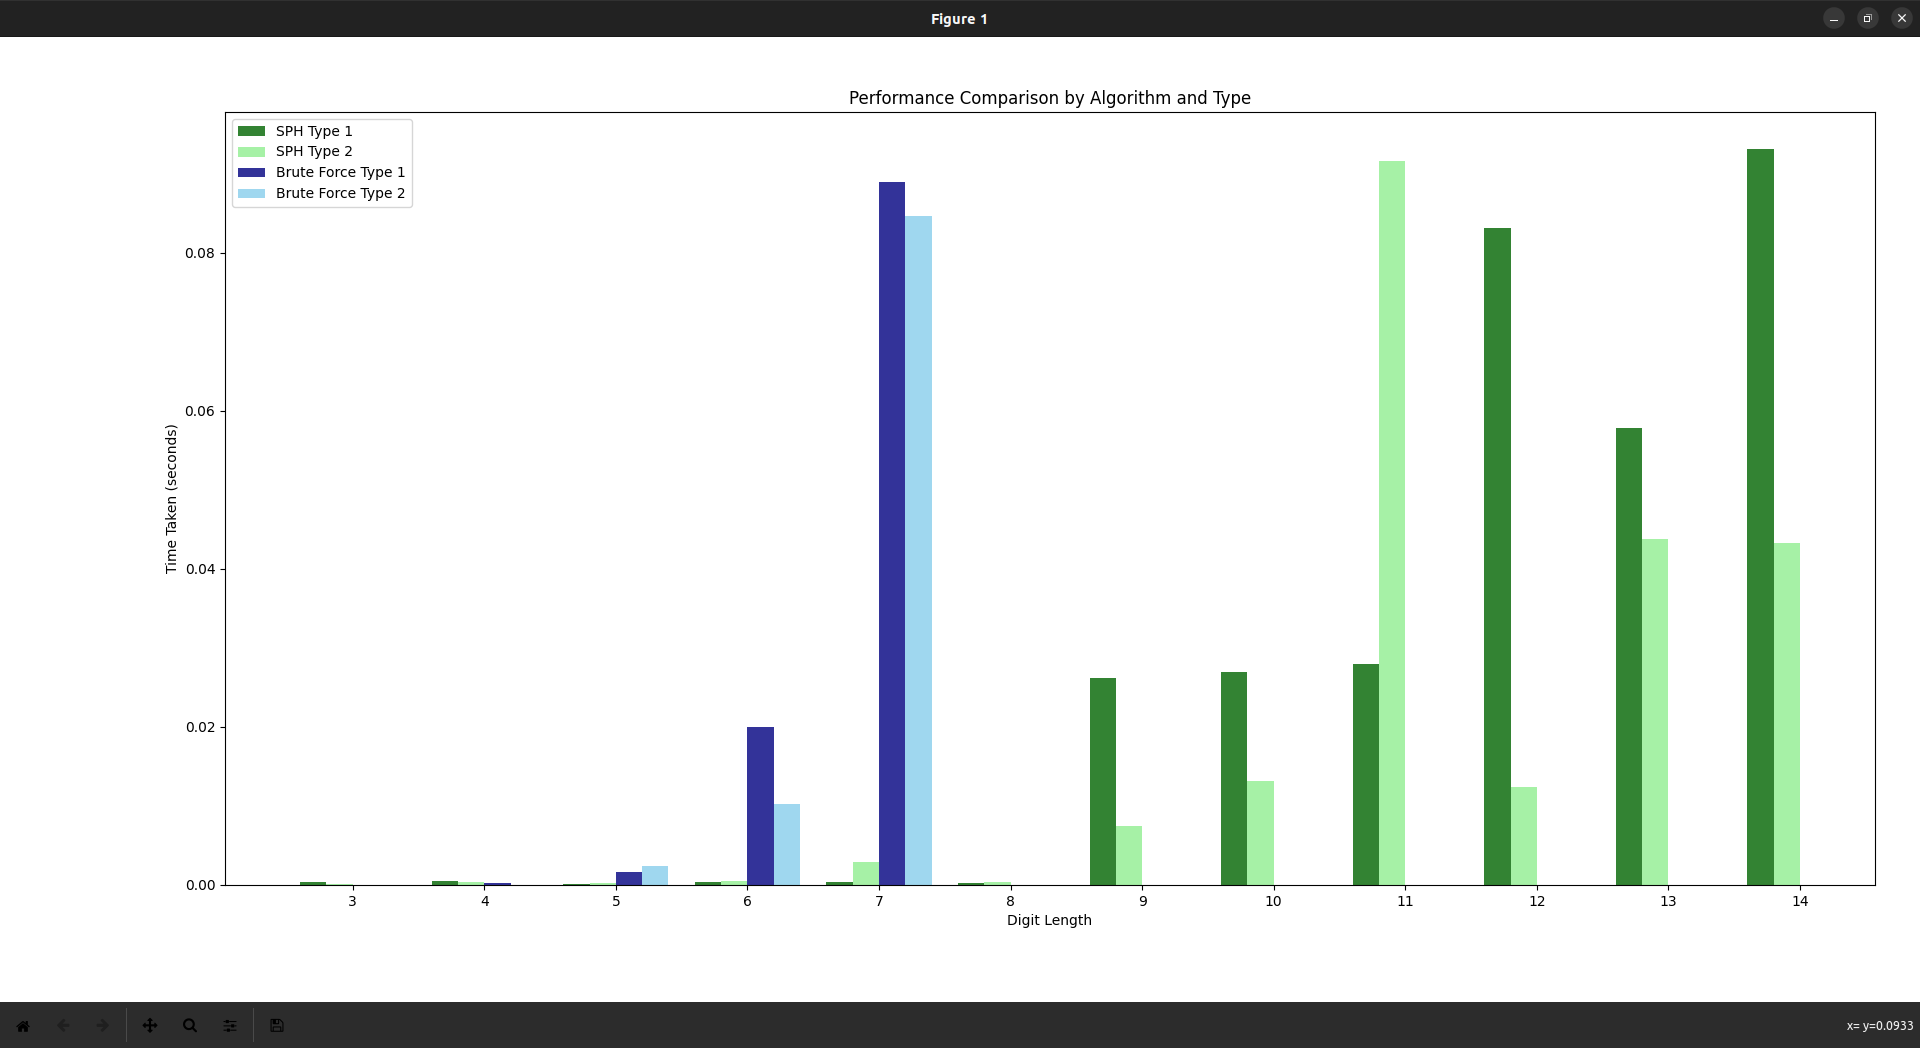
\includegraphics[width=1.0\textwidth]{time.png}
    \caption{час роботи}
    \label{fig:screenshot}
\end{figure}

\section{Висновок}
\quad
У цій роботі було розроблено програму для розв'язку задачі дискретного логарифму, автоматизовано заміри часу роботи розроблених алгоритмів, використовуючи надану програму, що генерує задачі різної довжини.
\end{document}
